\documentclass[sigconf, natbib=false]{acmart}

\def\BibTeX{{\rm B\kern-.05em{\sc i\kern-.025em b}\kern-.08emT\kern-.1667em\lower.7ex\hbox{E}\kern-.125emX}}

\usepackage{datetime2}
\usepackage{multirow}
\usepackage{amsmath}

\usepackage[style=ACM-Reference-Format,backend=bibtex,sorting=none]{biblatex}
\addbibresource{./refs.bib}

\usepackage{caption}
\usepackage{subcaption}
\usepackage{graphicx}
\graphicspath{{./figs/}}

\usepackage{listings, xcolor}

\newcommand{\JS}[1]{{\color{blue} [JS] #1}}
\newcommand{\RC}[1]{{\color{gray} [RC] #1}}
\newcommand{\HY}[1]{{\color{orange} [HY] #1}}

\newcommand{\TODO}[1]{{\color{red} [TODO] #1}}


\begin{document}
\title{
    Cross-Chain Payment (TODO) \\
    {\normalsize \normalfont version updated at \DTMnow }
}

\begin{abstract}
\TODO{}
\end{abstract}

\keywords{\TODO{}}

\maketitle

% Copyright 2017 Sergei Tikhomirov, MIT License
% https://github.com/s-tikhomirov/solidity-latex-highlighting/

\definecolor{verylightgray}{rgb}{.97,.97,.97}

\lstdefinelanguage{Solidity}{
	keywords=[1]{anonymous, assembly, assert, balance, break, call, callcode, case, catch, class, constant, continue, constructor, contract, debugger, default, delegatecall, delete, do, else, emit, event, experimental, export, external, false, finally, for, function, gas, if, implements, import, in, indexed, instanceof, interface, internal, is, length, library, log0, log1, log2, log3, log4, memory, modifier, new, payable, pragma, private, protected, public, pure, push, require, return, returns, revert, selfdestruct, send, solidity, storage, struct, suicide, super, switch, then, this, throw, transfer, true, try, typeof, using, value, view, while, with, addmod, ecrecover, keccak256, mulmod, ripemd160, sha256, sha3}, % generic keywords including crypto operations
	keywordstyle=[1]\color{blue}\bfseries,
	keywords=[2]{address, bool, byte, bytes, bytes1, bytes2, bytes3, bytes4, bytes5, bytes6, bytes7, bytes8, bytes9, bytes10, bytes11, bytes12, bytes13, bytes14, bytes15, bytes16, bytes17, bytes18, bytes19, bytes20, bytes21, bytes22, bytes23, bytes24, bytes25, bytes26, bytes27, bytes28, bytes29, bytes30, bytes31, bytes32, enum, int, int8, int16, int24, int32, int40, int48, int56, int64, int72, int80, int88, int96, int104, int112, int120, int128, int136, int144, int152, int160, int168, int176, int184, int192, int200, int208, int216, int224, int232, int240, int248, int256, mapping, string, uint, uint8, uint16, uint24, uint32, uint40, uint48, uint56, uint64, uint72, uint80, uint88, uint96, uint104, uint112, uint120, uint128, uint136, uint144, uint152, uint160, uint168, uint176, uint184, uint192, uint200, uint208, uint216, uint224, uint232, uint240, uint248, uint256, var, void, ether, finney, szabo, wei, days, hours, minutes, seconds, weeks, years},	% types; money and time units
	keywordstyle=[2]\color{teal}\bfseries,
	keywords=[3]{block, blockhash, coinbase, difficulty, gaslimit, number, timestamp, msg, data, gas, sender, sig, value, now, tx, gasprice, origin},	% environment variables
	keywordstyle=[3]\color{violet}\bfseries,
	identifierstyle=\color{black},
	sensitive=false,
	comment=[l]{//},
	morecomment=[s]{/*}{*/},
	commentstyle=\color{gray}\ttfamily,
	stringstyle=\color{red}\ttfamily,
	morestring=[b]',
	morestring=[b]"
}

\lstset{
	language=Solidity,
	backgroundcolor=\color{verylightgray},
	extendedchars=true,
	basicstyle=\footnotesize\ttfamily,
	showstringspaces=false,
	showspaces=false,
	numbers=left,
	numberstyle=\footnotesize,
	numbersep=9pt,
	tabsize=2,
	breaklines=true,
	showtabs=false,
	captionpos=b
}

\section{Introduction}
\label{sec:intro}

\HY{Indentions not so consistent.}\\
\HY{Space between paragraphs not so consistent.}

The Atomic Swap protocol is that two parties exchange \HY{(perform the exchange of?)} their assets ``atomically'' without trusted third parties \HY{(without any trusted thirdparty?)}.
``Atomic'' means the swap either succeeds or fails for both parties \HY{at any given time}.
Atomic Swap is implemented on blockchains by using the \HY{(remove "the"?)} Hashed Timelocked Contracts (HTLCs).
The HTLC is a type of transaction \HY{(contract?)} that, the payee should provide the preimage of a hash value before the deadline, otherwise the payment fails\HY{, and the payee will not receive the money}.

However, the fairness of the Atomic Swap is never studied formally.
First, there is no study that models the Atomic Swap in order to analyze whether both parties in the swap are equal.
Second, \HY{if having two parties reserving different rights, there is no research on the study of the risks they may encounter are equal, given that} the initiator in Atomic Swap can control the settlement time, while the asset price is fluctuating overtime.

In this paper, we prove that the Atomic Swap is unfair to the participant, and extends the original Atomic Swap \HY{protocol} to make it \HY{more} fair.
In particular, we formally model the Atomic Swap and the American Call Option in Finance,
and prove that the Atomic Swap is equivalent to a premium-free American Call Option.
Then we point out that the Atomic Swap is unfair to the participant, because the initiator is not required to pay for the premium \HY{, whereas it can speculate without any risk, making use of price fluctuations}.
Based on this observation, we evaluate the unfairness of the Atomic Swap by estimating how much the premium should be for mainstream cryptocurrency pairs.
Estimating the premium is based on the Cox-Ross-Rubinstein option pricing model in Finance, which is a conventional model to price the American-style options.
% TODO evaluation result
After that, we propose two fair Atomic Swap protocols, which implement the premium mechanism upon the original Atomic Swap protocols.
One of the protocols is for the currency exchange, and the other is for the American Call Options.
Both protocols can be deployed on existing blockchains:
They can be directly deployed on blockchains supporting smart contracts (e.g. Ethereum),
and can be deployed on blockchains supporting scripts (e.g. Bitcoin) by adding a single opcode.

Our contributions are as follows:

\paragraph{We formalize the Atomic Swap and the American Call Option, and prove that the Atomic Swap is equivalent to the premium-free American Call Option.\HY{"a... is a..."?}} 
We use formal languages to define the Atomic Swap and the American Call Option.
In particular, we describe them as protocols, and prove that the Atomic Swap is equivalent to the premium-free American Call Option:
The initiator and the participant in Atomic Swap are the option buyer and the option seller in American Call Options, respectively;
The initiator asset and the participant asset in Atomic Swap are the used currency and the underlying asset in American Call Options, respectively;
The participant asset's timelock in Atomic Swap is the strike time in American Call Options;
The current price of the participant asset in Atomic Swap is the strike price in American Call Options;
Redeeming cryptocurrencies in Atomic Swap is exercising the contract in the American Call Options.

\paragraph{We observe that the Atomic Swap is unfair to the particiapant due to the unpaid premium, and evaluate its unfairness by estimating the premium for mainstream cryptocurrency pairs.}
We point out that according to the option theory in Finance, the Atomic Swap - modelled as the premium-free American Call Option - is unfair to the participant, especially in the highly volatile cryptocurrency market.
In practice, the initiator can decide whether to swap based on the exchange rate trend: If his asset price falls, he will exercise the contract, otherwise he can wait for the contract to expire.
In this way, the initiator is risk-free towards the cryptocurrency market. 
We then evaluate the unfairness of the Atomic Swaps for mainstream cryptocurrency paris.
Our evaluation consists of two parts: the volatility analysis and the premium pricing.
First, we analyze the exchange rate volatility of mainstream cryptocurrency pairs, in order to reveal how much reward the initiator can get and how much risk the initiator can delegate to the participant.
Second, we estimate how much the premium should be, by using the Cox-Ross-Rubinstein option pricing model.
The Cox-Ross-Rubinstein model is the conventional option pricing model for American-style options.
By estimating the premium, we can reveal how unfair the Atomic Swap is.

\paragraph{We propose two fair Atomic Swap protocols, one is for currency exchange and the other is for American Call Options.}
Based on our observation that the unfairness is introduced by the unpaid premium,
we then propose two fair Atomic Swap protocols, one is for currency exchange and the other is for American Call Options.
The two protocols achieve the fairness by implementing the premium mechanism upon the original protocol - The initiator should deposit the premium on the participant's blockchain when initiating the swap.
In the currency exchange-style protocol, if the swap is successful, the premium goes back to the initiator, otherwise it goes to the participant.
In the American Call Option-style protocol, the premium goes to the participant once the participant's asset is redeemed or refunded.

\paragraph{We describe how to deploy our proposed protocols on existing blockchains.}
We give solutions to deploy our protocols on existing blockchains, including blockchains supporting smart contracts and blockchains supporting scripts only.
For blockchains supporting smart contracts such as Ethereum, our protocols can be directly deployed.
For blockchains only supporting scripts such as Bitcoin, our protocols can be deployed by adding one more opcode.
We call the opcode ``OP\_LOOKUP\_OUTPUT'', and it looks up the owner of a specific output.
We use Solidity as an example of smart contracts, and the Bitcoin script code as an example of scripts.

The paper is structured as follows.
Section~\ref{sec:background} describes the background of Atomic Swap and options in Finance.
Section~\ref{sec:formalization} formalizes the Atomic Swap protocol and the American Call Option, then proves the Atomic Swap protocol is equivalent to the premium-free American Call Option.
Section~\ref{sec:evaluation} evaluates the Atomic Swap unfairness by analyzing the volatility and pricing the premium of mainstream cryptocurrency pairs.
Section~\ref{sec:fair_atomic_swap} describes our proposed fair Atomic Swap protocols.
Section~\ref{sec:deployment} describes how to deploy our proposed protocols on existing blockchains.
Section~\ref{sec:discussion} discusses security issues of Atomic Swaps, other countermeasures for solving the Atomic Swap unfairness, and limitations of our protocols.
Section~\ref{sec:conclusion} concludes our paper and outlines the future work.
\section{Background}
\label{sec:background}

\subsection{Atomic Cross-chain Swap}

\subsection{Option}

% option

% american option and european option

% call option and put option

% premium fee
\section{Formalization}
\label{sec:formalization}

In this section, we formalize the Atomic Swap protocol \MOD{(the original version on Bitcointalk~\cite{nolan2013alt})} and the American Call Option,
then prove that the Atomic Swap is equivalent to an American Call Option without the premium.



\begin{figure}
    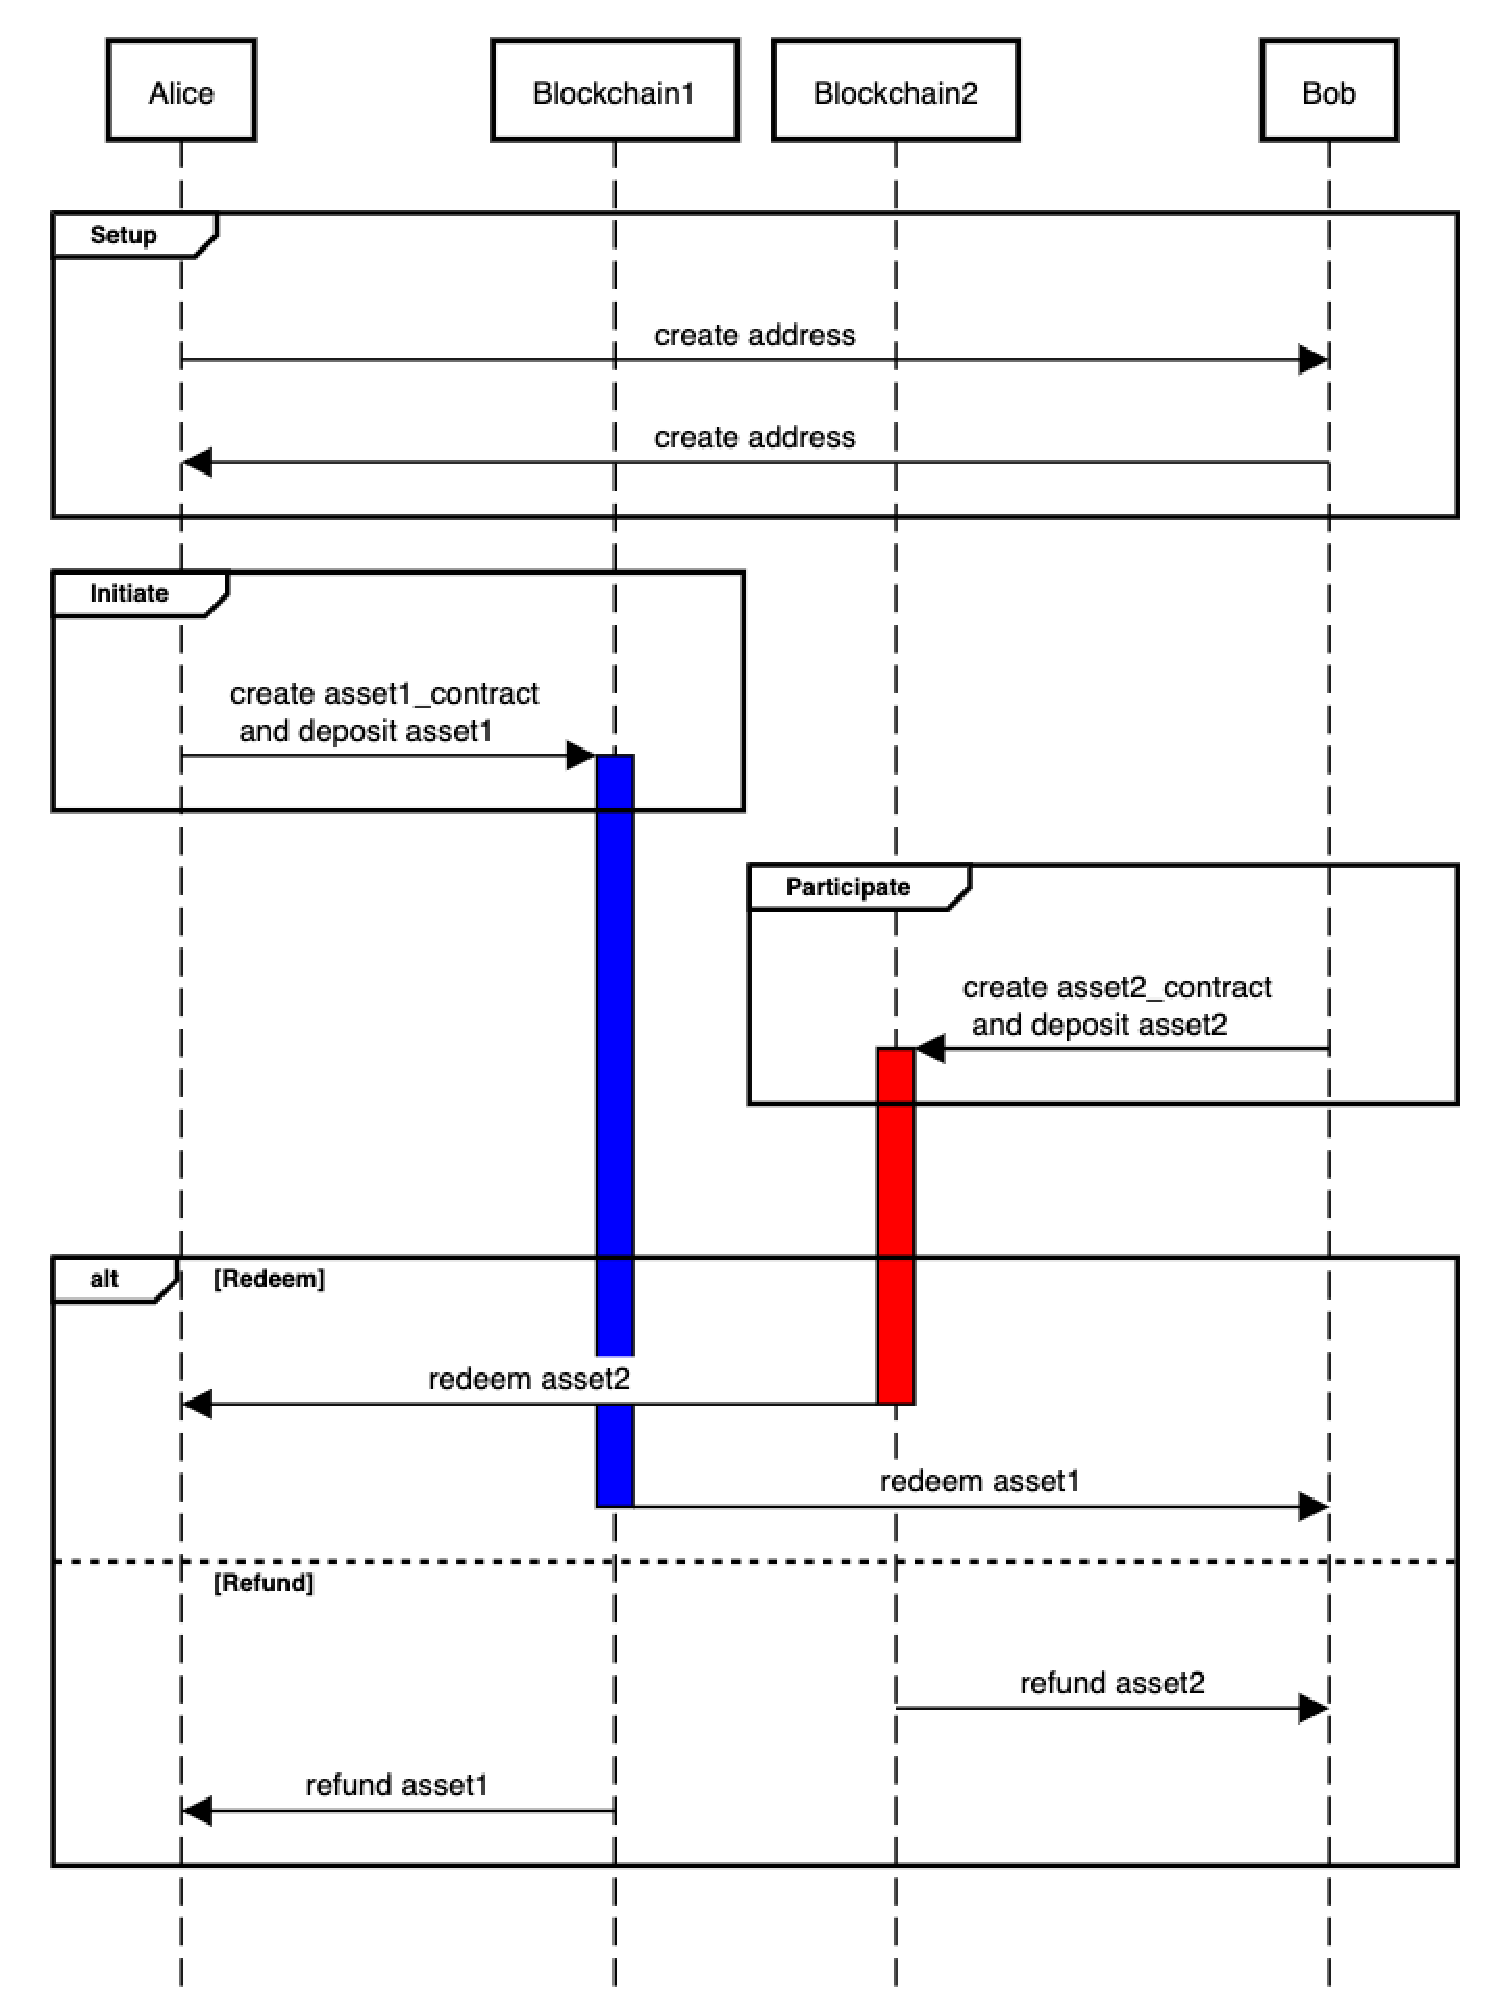
\includegraphics[width=.7\linewidth]{sequence_diagram_original.eps}
    \caption{Sequence diagram of the Atomic Swap.}
    \label{fig:sequence_diagram_original}
\end{figure}

\begin{figure}
    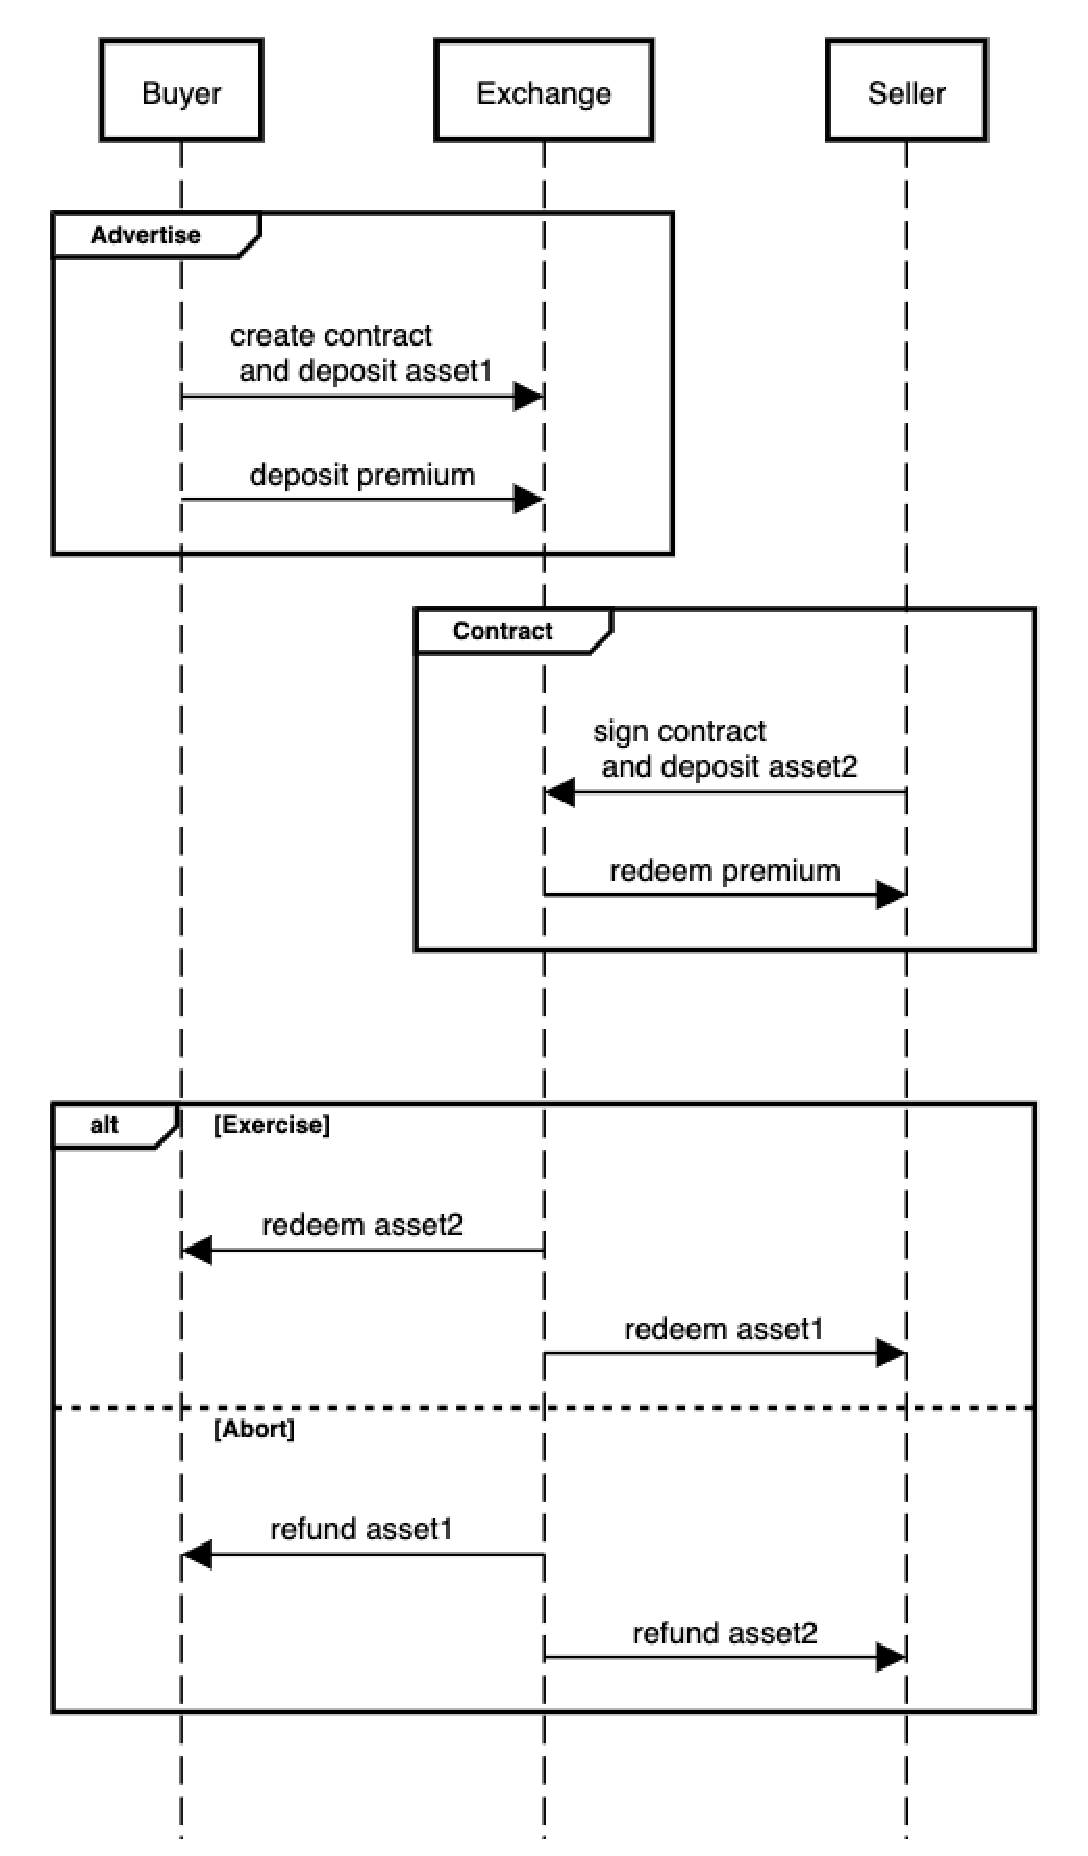
\includegraphics[width=.7\linewidth]{sequence_diagram_option.eps}
    \caption{Sequence diagram of the American Call Option.}
    \label{fig:sequence_diagram_option}
\end{figure}





\subsection{Atomic Swap}

\MOD{We formalise the original version of the Atomic Swap~\cite{nolan2013alt}.

\subsubsection{Security assumptions}

Before the formalization, we give security assumptions on the Atomic Swap.

First, we assume blockchains involved in the Atomic Swap are secure.
The Atomic Swap is based on blockchains.
If the blockchains are insecure, the Atomic Swap will also be insecure.

Second, we assume the HTLC mechanism in blockchains is reliable.
More specifically,
1) blockchains produce new blocks with stable speeds;
2) the hash algorithm used by HTLCs is secure;
3) the runtime for executing HTLCs is reliable.


Third, the time for confirming a transaction is negligible compared to timelocks.
In practice, the swap initiator's timelock is 48 hours and the swap participant's timelock is 24 hours by default~\cite{nolan2013alt}, while confirming a transaction is less than 1 hour for most blockchains.

}

\subsubsection{Process}

We denote the initiator in the Atomic Swap as Alice, and the participant as Bob.

\begin{definition}
We define an Atomic Swap $\mathcal{AS}$ as

$$\mathcal{AS} = (x_1, Coin_1, x_2, Coin_2)$$

where Alice hopes to buy $x_2$ $Coin_2$ on blockchain $BC_2$ from Bob with $x_1$ $Coin_1$ on blockchain $BC_1$.
\end{definition}

The Atomic Swap protocol consists of five algorithms:
\textbf{Setup},
\textbf{Initiate},
\textbf{Participate},
\textbf{Redeem}, and
\textbf{Refund}.

\TODO{rewrite all formalization! lacks parameters!}

\paragraph{\textbf{Setup}($k$)}
\textbf{Setup}($\cdot$) takes a security parameter $k$,
and returns the addresses on two blockchains for both Alice and Bob $\beta_{A, 1}$, $\beta_{A, 2}$, $\beta_{B, 1}$, $\beta_{B, 2}$.

\paragraph{\textbf{Initiate}($\beta_{B, 1}, x_1$)}
\textbf{Initiate}($\cdot$) takes Bob's address $\beta_{B, 1}$ on $BC_1$ and the amount $x_1$ of Alice's $Coin_1$,
and returns the preimage $s$, the hash $h$, the contract script $\mathcal{C}_1$, the contract transaction $tx_{\mathcal{C}, 1}$, the refund script $\mathcal{R}_1$, and the refund transaction $tx_{\mathcal{R}, 1}$.
The preimage $s$ is a random string generated by Alice. At this stage, $s$ is only known to Alice.
The preimage hash $h = \mathcal{H}(s)$, where $\mathcal{H}$ is a secure hash function.
$h$ is published when triggering \textbf{Initiate}($\cdot$).
The contract script $\mathcal{C}_1$ is that ``Alice pays $x_1$ $Coin_1$ from $\beta_{A, 1}$ to $\beta_{B, 1}$ if Bob can provide $s$ before or on a timelock $\delta_1$ (which is a timestamp). After $\delta_1$, Alice can refund the money - get $x_1$ $Coin_1$ back.''
$\mathcal{C}_1$ will be published as a transaction $tx_{\mathcal{C}, 1}$ on $BC_1$ when triggering \textbf{Initiate}($\cdot$).
The refund script $\mathcal{R}_1$ is that ``Alice pays $x_1$ $Coin_1$ from $\beta_{A, 1}$ to her another address.'' This is to ensure $x_1$ $Coin_1$ can no longer be redeemed by others. Alice can do this only after $\delta_1$.
The refund is done by publishing $\mathcal{R}_1$ as a transaction $tx_{\mathcal{R}, 1}$ on $BC_1$ if Alice can and decide to refund.

\paragraph{\textbf{Participate}($\beta_{A, 2}, x_2, h$)}
\textbf{Participate}($\cdot$) takes Alice's address $\beta_{A, 2}$ on $BC_2$, the amount $x_2$ of Bob's $Coin_2$ and the hash $h$,
and returns the contract script $\mathcal{C}_2$, the contract transaction $tx_{\mathcal{C}, 2}$, the refund script $\mathcal{R}_2$, and the refund transaction $tx_{\mathcal{R}, 2}$.
The contract script $\mathcal{C}_2$ is that ``Bob pays $x_2$ $Coin_2$ from $\beta_{B, 2}$ to $\beta_{A, 2}$ if Alice can provide $s$ before or on a timelock $\delta_2$ (which is a timestamp). After the time of $\delta_2$, Bob can refund the money - get $x_2$ $Coin_2$ back.''
Here $\delta_2$ should expire earlier than $\delta_1$.
The contract script is published as a transaction $tx_{\mathcal{C}, 2}$ on $BC_2$ when triggering \textbf{Initiate}($\cdot$).
The refund script $\mathcal{R}_2$ is that ``Bob pays $x_2$ $Coin_2$ from $\beta_{B, 2}$ to his another address.'' This is to ensure $x_2$ $Coin_2$ can no longer be redeemed by others. Bob can do this only after $\delta_2$.
The refund is done by publishing $\mathcal{R}_2$ as a transaction $tx_{\mathcal{R}, 2}$ on $BC_2$ if Bob can and decide to refund.

\paragraph{\textbf{Redeem}($s$)}
\textbf{Redeem}($\cdot$) takes the preimage $s$,
and returns $\mathcal{V} \in \{0, 1\}$ indicating if the redemption is successful or not.
The redemption can be performed by both parties, and Alice should redeem earlier than Bob.
As Alice knows $s$, she can redeem $x_2$ $Coin_2$ - pay $x_2$ $Coin_2$ in $\beta_{A, 2}$ to her another address by attaching $s$ in this transaction.
After Alice redeems $x_2$ $Coin_2$, $s$ is published and revealed to everyone including Bob, so that Bob can redeem $x_1$ $Coin_1$, similarly.

\paragraph{\textbf{Refund}()}
\textbf{Refund}($\cdot$) takes no parameters and returns the $\mathcal{V} \in \{0, 1\}$ indicating if the refund is successful or not.
Alice and Bob can perform the refund by publishing $tx_{\mathcal{R}, 1}$ and $tx_{\mathcal{R}, 2}$ after the timelock $\delta_1$ and $\delta_2$, respectively.

% procedure
\paragraph{Process.}
Figure~\ref{fig:sequence_diagram_original} shows the Atomic Swap process.
More specifically, Alice and Bob proceeds the Atomic Swap as follows:
Alice and Bob first creates addresses by triggering \textbf{Setup}($\cdot$).
Alice then triggers \textbf{Initiate}($\cdot$) to initiate the swap $\mathcal{AS}$, and Bob triggers \textbf{Participate}($\cdot$) to participate in $\mathcal{AS}$.
Within $\delta_2$ Alice can redeem $x_2$ $Coin_2$ by triggering \textbf{Redeem}($\cdot$), then Bob can redeem $x_1$ $Coin_1$ by triggering \textbf{Redeem}($\cdot$).
In this case, $\mathcal{AS}$ succeeds for both Alice and Bob.
However, Alice can also keep not triggering \textbf{Redeem}($\cdot$) and wait for $\delta_2$ to expire.
After $\delta_2$ expires, Bob can refund $x_2$ $Coin_2$ by triggering \textbf{Refund}($\cdot$), and Alice can refund $x_1$ $Coin_1$ by triggering \textbf{Refund}($\cdot$) after $\delta_1$ expires.
In this case, $\mathcal{AS}$ fails for both Alice and Bob.

% why atomic
We can see that $\mathcal{AS}$ either succeeds or fails for both Alice and Bob.
In detail,

\begin{itemize}
    \item If Alice misbehaves when triggering \textbf{Setup}($\cdot$) or \textbf{Initiate}($\cdot$), Bob will lose nothing as he hasn't deposited $Coin_2$ yet.
    \item If Bob misbehaves when triggering \textbf{Participate}($\cdot$), Alice can choose to abort $\mathcal{AS}$ by triggering \textbf{Refund}($\cdot$).
    \item Alice can only choose to \textbf{Redeem}($\cdot$) $Coin_2$ or wait $\delta_2$ to expire.
    Once Alice triggers \textbf{Redeem}($\cdot$), Bob can also trigger \textbf{Redeem}($\cdot$).
    Once $\delta_2$ expires, Bob can trigger \textbf{Refund}($\cdot$) to get his $x_2$ $Coin_2$ back.
\end{itemize}

% misuse
However, one may take both $Coin_1$ and $Coin_2$ if the other does not trigger \textbf{Redeem}($\cdot$) or \textbf{Refund}($\cdot$) on time.
For example, if Bob does not trigger \textbf{Redeem}($\cdot$) after Alice triggers \textbf{Redeem}($\cdot$) and $\delta_1$ expires, Alice can also refund $x_1$ $Coin_1$ by triggering \textbf{Refund}($\cdot$).
But in this case it is Bob to blame, because he should have had enough time - at least $\delta_2 - \delta_1$ \MOD{(48 - 24 = 24 hours by default)} - to redeem $x_1$ $Coin_1$.
Another example is that Alice broadcasts the transaction of \textbf{Redeem}($\cdot$) after $\delta_2$, but Bob has already triggered \textbf{Refund}($\cdot$).
Therefore, Bob can also trigger \textbf{Redeem}($\cdot$) with the preimage in Alice's transaction of \textbf{Redeem}($\cdot$) before $\delta_1$.
Similarly, it is Alice to blame, because she should have had enough time - before $\delta_2$ - to trigger \textbf{Redeem}($\cdot$).

% def S_t
Similar to conventional finance assets, $Coin_2$'s value is also fluctuating due to the market mechanism.
We denote the asset's underlying value (with the unit $\frac{Coin_2}{Coin_1}$) at the time $t$ as $S_t$.















\subsection{American Call Option}

The American Call Option is a contract that ``one can buy an amount of an asset with an agreed price prior to or on an agreed time in the future''. 
The agreed price is usually called the \textit{spot price}, and the buying is called \textit{exercising}.
For American Call Option, the option buyer can exercise in advanced of the agreed exercise time.
The price of the asset when exercising is called the \textit{strike price}.
As mentioned in Section~\ref{subsec:background_option}, the option contract itself has value, and its value is called the \textit{premium}.
The option buyer should pay for both the asset and the premium when participating in the contract.

Formally,

\begin{definition}
We define an American Call Option contract $\Pi$ as

$$\Pi = (\pi_1, \pi_2, K, A, T, C)$$

where
$\pi_1$ and $\pi_2$ are the currency of the option buyer and the asset of the option seller, respectively; 
$K$ is the strike price with the unit $\pi_2 / \pi_1$ \HY{isnt it  $\pi_1 / \pi_2$?}- the price of $\pi_2$ measured in $\pi_1$;
$A$ is the amount of the asset $\pi_2$ that the option seller wants to sell;
$T$ is the agreed strike time;
$C$ is the \textit{premium} with the unit $\pi_1$.
\end{definition}

The process of an American Call Option is as follows:

\begin{enumerate}
    \item \textbf{Advertise}: The option seller creates and advertises an American Call Option contract $\Pi = (\pi_1, \pi_2, K, A, T, C)$.
    \item \textbf{Contract}: The option buyer finds $\Pi$ is profitable, so he participates in $\Pi$.
    To participate, the option buyer should pay $C$ to the option seller first.
    Note that the option buyer does not pay for $A$ $\pi_2$ at this stage.
    Also note that the option seller cannot abort $\Pi$ after the option buyer participates in $\Pi$.
    \item \textbf{Exercise} or \textbf{Abort}: The option buyer exercises $\Pi$ - pays $AK$ $\pi_1$ to the option seller - before or on $T$, and the option seller gives $A$ $\pi_2$ to the option buyer.
    If the option buyer does not exercise $\Pi$ before or on $T$, $\Pi$ will abort - the option buyer gets $\pi_1$ back and the option seller gets $\pi_2$ back and $C$. In other words, both of them get their underlying asset back, but the option buyer loses the premium $C$.
\end{enumerate}

% asset underlying value
The underlying value of $\pi_2$ is fluctuating over time due to the market mechanism.
Intuitively, if the price of $\pi_2$ rises when the option buyer exercises $\Pi$, the option buyer profits, because he buys $\pi_2$ with the price lower than the current market price.
Formally, we denote the asset's underlying value (with the unit $\pi_2 / \pi_1$) at the time $t$ as $S_t$.
Assume the option buyer exercises $\Pi$ at a time $T' \leq T$, he can profit $[(S_{T'} - K) A - C]$ $\pi_1$.













\subsection{An Atomic Swap is a premium-free American Call Option}

We show that an Atomic Swap is equivalent to a premium-free American Call Option.

More specifically,

\begin{theorem}
$\mathcal{AS} = (x_1, Coin_1, x_2, Coin_2)$ is equivalent to the American Call Option contract

$$
\Pi = (Coin_1, Coin_2, \frac{x_2}{x_1}, x_2, \delta_2, 0)
$$

where:
\textbf{Advertise} in the American Call Option is equivalent to \textbf{Setup}($\cdot$) and \textbf{Initiate}($\cdot$) in the Atomic Swap;
\textbf{Contract} in the American Call Option is equivalent to \textbf{Participate}($\cdot$) in the Atomic Swap;
\textbf{Exercise} in the American Call Option is equivalent to \textbf{Redeem}($\cdot$) in the Atomic Swap;
\textbf{Abort} in the American Call Option is equivalent to \textbf{Refund}($\cdot$) in the Atomic Swap.

\end{theorem}


\begin{proof}

In the American Call Option context, the option buyer Alice wants to buy $x_2$ $Coin_2$ from the participant Bob by using $x_1$ $Coin_1$.
$Coin_1$ is the currency Alice uses, $Coin_2$ is the asset Bob has.
$\frac{x_2}{x_1}$ is the price of the asset from Alice's perspective, so $\frac{x_2}{x_1}$.
$\delta_2$ is the timelock of the contract transaction on $BC_2$.
It is equivalent to the strike time of $\Pi$, because after $\delta_2$ Bob can refund his asset back and invalidate $\mathcal{AS}$, but before $\delta_2$ Bob cannot abort $\mathcal{AS}$ if Alice \textbf{Participate}s.
Establishing the Atomic Swap does not require Alice to pay anything other than the asset to Bob, so the premium here is zero.
\end{proof}
\section{Evaluating the Unfairness of Atomic Cross-Chain Swaps}
\label{sec:evaluation}

\subsection{Intuitive Analysis}

\subsection{Volatility Analysis}

\subsection{Mitigated Risk of the Initiator}
\section{Fair Atomic Swaps}
\label{sec:fair_atomic_swap}

In this section, we propose an improvement on the original Atomic Swap to make it fair.
It implements the premium mechanism, and supports both the currency exchange-style Atomic Swap and the American Call Option-style Atomic Swap.


\subsection{Design}

\subsubsection{Difference between Currency Exchange and Options}
\label{subsubsec:diff_spot_option}

We first summarise the design objectives for Atomic Swap.

To our knowledge, the Atomic Swap protocol is originally designed for the fair exchange between different cryptocurrencies.
However, according to our analysis, the protocol is unfair due to the Optionality and the free premium.
Also, for (crypto)currency exchange, the protocol should have no Optionality.
The currency exchange and the American Call Option differ in Finance: the currency exchange is a type of Spots~\cite{hull1991introduction}, while the American Call Option is a type of Options.
The Spot Contract and the Option Contract aim at different application scenarios: the Spot Contract aims at exchanging the ownership of assets, while the Option Contract aims at providing Alice an ``option'' to trade.
More specifically, Spots and Options differ in the following aspects:

\begin{itemize}
    \item The Spot Contract is exercised immediately, while the Option Contract is exercised on or prior to a specified date in the future.
    \item The Spot Contract cannot be aborted once signed by both parties, while in the Option Contract Alice can abort the contract with the loss of the premium.
    \item The Spot Contract itself has no value, while the Option Contract itself has value - the premium.
\end{itemize}

\subsubsection{Premium for Currency Exchange and American Call Options}
\label{subsubsec:design_obj}

According to Section~\ref{subsubsec:diff_spot_option}, the currency exchange-style Atomic Swaps and the American Call Option-style Atomic Swaps differ in design objectives.

\paragraph{Atomic Swaps for Currency Exchange}
For the currency exchange, both parties are not permitted to abort the contract once signed.
However, in Atomic Swaps, Alice can abort the swap by not releasing the random secret.
Therefore, the protocol should discourage Alice to abort the swap.
To achieve this, we can use the premium mechanism as the collateral: Alice should deposit the premium besides her asset when \textbf{Initiate}.
The premium should follow that:
\textbf{Alice pays the premium to Bob if Bob refunds his asset after his timelock but before Alice's timelock.
If Alice's timelock expires, Alice can refund her premium back.}

\paragraph{Atomic Swaps for American Call Options}
For the American Call Options, Alice should pay for the premium besides the underlying asset, regardless of whether the swap is successful or not.
In reality, the option sellers are trustworthy - the option sellers never abort the contract.
However, in Atomic Swaps, Bob can abort the contracts like Alice.
To keep the Atomic Swap consistent with the American Call Options,
the premium should follow that: 
\textbf{Alice pays the premium to Bob if
1) Alice redeems Bob's asset before Bob's timelock, or
2) Bob refunds his asset after Bob's timelock but before Alice's timelock.
If Alice's timelock expires, Alice can refund her premium back.}











\subsection{Our protocol}


\begin{figure}[htp]
    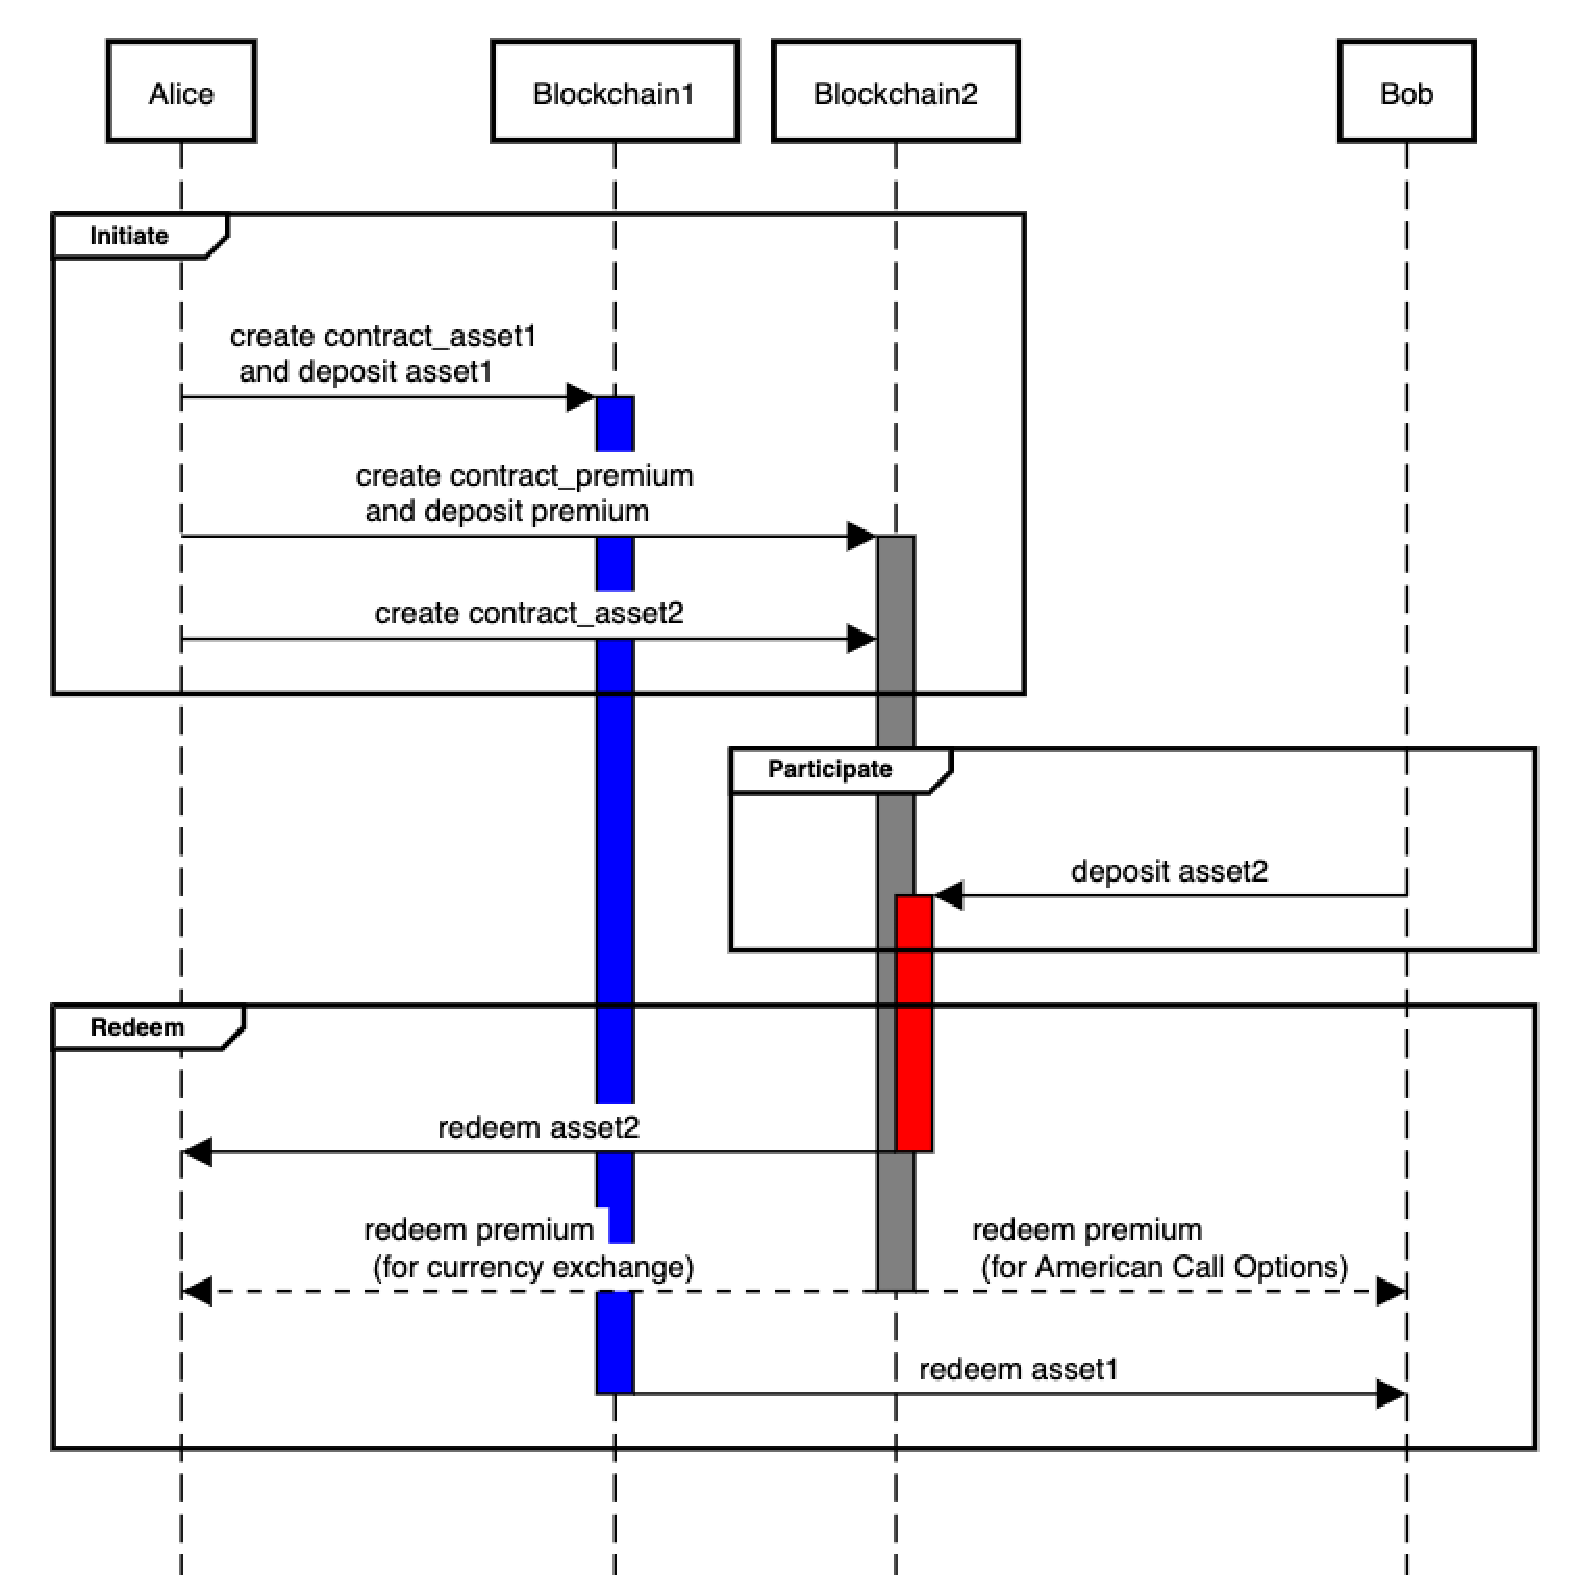
\includegraphics[width=.9\linewidth]{sequence_diagram_us.eps}
    \caption{Sequence diagram of our Atomic Swap.
    For currency exchange-style Atomic Swaps, the premium will go back to Alice if the swap is successful (the left dotted line).
    For American Call Option-style Atomic Swaps, the premium will go to Bob if the swap is successful (the right dotted line).}
    \label{fig:sequence_diagram_us}
\end{figure}

We propose an improvement on the Atomic Swap, which implements the premium mechanism, to make it fair.
It can fulfill design objectives of both the currency exchange and the American Call Option.
Figure~\ref{fig:sequence_diagram_us}) shows the process of our Atomic Swap.

We denote our Atomic Swap protocol $\mathcal{AS}'$ as

$$\mathcal{AS}' = (x_1, Coin_1, x_2, Coin_2, pr)$$

where $pr$ is the amount of the premium measured in $Coin_2$.
In our protocol, besides $x_1$ $Coin_1$, Alice should also lock $pr$ $Coin_2$ on $BC_2$, which will be described later.

Similar to the original Atomic Swap $\mathcal{AS}$, our protocol consists of four stages:
\textbf{Initiate}, \textbf{Participate}, \textbf{Redeem} and \textbf{Refund}.

\paragraph{\textbf{Initiate}}
Different from $\mathcal{AS}$, Alice also creates Bob's contract script $\mathcal{C}_2$ and its associated transaction $tx_{\mathcal{C}, 2}$ when \textbf{Initiate} in $\mathcal{AS}'$.

$\mathcal{C}_1$ and $tx_{\mathcal{C}, 1}$ is the same as in $\mathcal{AS}$,
while $\mathcal{C}_2$ and $tx_{\mathcal{C}, 2}$ are more sophisticated.
$\mathcal{C}_2$ contains two coherent sub-contracts $\mathcal{C}^{asset}_2$ and $\mathcal{C}^{pr}_2$.

In $\mathcal{C}_2$, $\mathcal{C}^{asset}_2$ is the contract for the asset $x_2$ $Coin_2$, which is the same as in $\mathcal{AS}$.
$\mathcal{C}^{pr}_2$ is the contract for the premium $pr$, which implements the premium mechanism in the Atomic Swap.
It supports both the currency exchange-style Atomic Swap and the American Call Option-style Atomic Swap.
In more detail, the rules of $\mathcal{C}^{pr}_2$ are shown below:

\begin{description}
    \item[$\mathcal{C}^{pr}_2$ for currency exchange] Alice pays $pr$ to Bob with the condition:
    Bob refunds $x_2$ $Coin_2$ after $\delta_2$ and before $\delta_1$.
    If $\delta_1$ expires, Alice can refund $pr$ back.
    \item[$\mathcal{C}^{pr}_2$ for American Call Options] Alice pays $pr$ to Bob with one of the two conditions:
    1) Alice redeems $x_2$ $Coin_2$ before $\delta_2$.
    2) Bob refunds $x_2$ $Coin_2$ after $\delta_2$ but before $Delta_1$ (note that $\delta_2 < \delta_1$).
    If $\delta_1$ expires, Alice can refund $pr$ back.
\end{description}

Alice published $tx_{\mathcal{C}, 1}$ on $BC_1$ and $tx_{\mathcal{C}, 2}$ on $BC_2$.
Note that Alice only triggers $\mathcal{C}_1$ and $\mathcal{C}^{pr}_2$ to execute at this stage.
Bob will deposit $x_2$ $Coin_2$ trigger $\mathcal{C}^{asset}_2$ to execute when \textbf{Participate}.

\paragraph{\textbf{Participate}}
Bob decides whether to participate in $\mathcal{AS}'$ by auditing $tx_{\mathcal{C}, 1}$ and $tx_{\mathcal{C}, 2}$.
If Bob thinks contracts are fair, he will participate in $\mathcal{AS}'$, otherwise Bob will not participate and look for more profitable contracts from others.
To participate in $\mathcal{AS}'$, Bob deposits $x_2$ $Coin_2$ in $\mathcal{C}^{asset}_2$, and triggers $\mathcal{C}^{asset}_2$ to execute.

\paragraph{\textbf{Redeem}}
Alice redeeming $x_2$ $Coin_2$ and Bob redeeming $x_1$ $Coin_1$ are the same in $\mathcal{AS}'$ and $\mathcal{AS}$.
But in addition, riles in $\mathcal{C}^{pr}_2$ will work once triggering \textbf{Redeem} for $\mathcal{AS}'$.

\paragraph{\textbf{Refund}}
Refunding $x_1$ $Coin_1$ for Alice and $x_2$ $Coin_2$ for Bob are the same as in $\mathcal{AS}$.
But in addition, rules in $\mathcal{C}^{pr}_2$ will work once triggering \textbf{Refund} for $\mathcal{AS}'$.
\section{Deployment}
\label{sec:deployment}

\subsection{Atomic Swaps for Currency Exchange}

% can implement the currency exchange by ifelse
% smart contracts can, script cannot
% reason: redeem can be signalled by the pre-image release
%   refund cannot be signalled or verified


\subsection{Atomic Swaps for American Call Options}

% can implement the American Call Options by hashlock or by ifelse
% script and smart contracts

\section{Discussion}
\label{sec:discussion}

\subsection{Security of Atomic Swap}

Although already widely adopted, Atomic Swap has security issues.

% rely on blockchain security
First, the security of Atomic Swaps relies on the security of blockchains:
if the blockchains involved in the swaps are insecure, the Atomic Swaps will also be insecure.

% smart contract /script
Second, the Atomic Swap contracts are written in high-level languages, so the compiled contracts can be insecure if the contract compilers are flawed.

% 2 blockchain async
Third, the timelock is unreliable in the cross-chain scenario.
Similar to other distributed systems~\cite{coulouris2012distributed}, different blockchains are unsynchronised on the time.
% timestamp of blockchain
Blockchains timestamp events by either two approaches: using the block height or using the UNIX timestamp.
% relative time
The block height can serialise events on a blockchain by time, but cannot serialise events outside the blockchain.
In addition, the new block generation is a random process, so the block height cannot indicate the precise time in reality.
% abosolute time
Using the UNIX timestamp doesn't work, either.
This is because the consensus participants are responsible for timestamping events, but the consensus participants can be unreliable:
they may use the wrong time, either on purpose or by accident.


\subsection{Other countermeasures}

Besides our proposal, there are some other countermeasures to address the Atomic Swap unfairness.
Unfortunately, to our knowledge, all of them either have security flaws or significantly reduce the usability of Atomic Swaps.

The first countermeasure is to make Atomic Swap costly by charging setting up HTLCs, or increasing the transaction fee of HTLCs.
However, these two solutions do not only significantly reduce the usability of Atomic Swaps, but also affect HTLCs not aiming at setting up Atomic Swaps.

The second solution is to use shorter timelock for Atomic Swaps.
Unfortunately, short timelocks may cause unexpected consequences.
Confirming transactions for setting up Atomic Swaps takes time, and the time required is highly unpredictable.
With short timelocks, the transactions for setting up Atomic Swaps may be confirmed after the expiration of timelocks.

The third solution is to use a trusted third party (TTP) to implement the premium mechanism.
When Alice initiates an Atomic Swap, the TTP forces Alice to deposit the premium.
Although this TTP does not require Alice and Bob to escrow their assets, the TTP should be trustworthy and can be a single point of failure.

\subsection{Limitations of our protocols}

Still, our solutions are not perfect.
% should hold asset
The initiators of Atomic Swaps need to hold some participant's asset to initiate an Atomic Swap,
for either collateralising successful swaps or paying for the option itself.
Unfortunately, the initiators do not always have participant's asset: they may just hope to get some participant's asset with only his asset.
Before doing an Atomic Swap, the initiator should get some participant's asset by arbitrary means.
For example, he can buy some participant's asset from cryptocurrency exchanges, or initiate a smaller Atomic Swap with shorter timelocks and no premium.
% option seller cannot change premium in our protocols
Also, in an exchange, the option seller can change the premium at any given time until the option buyer signs the option agreement, while in our protocols the option seller cannot update the premium after publishing the option contract.
In this way, the original Atomic Swap protocol and our protocols are less efficient than centralised solutions in terms of the market liquidity.
\section{Related Work}
\label{sec:related_work}

\paragraph{Atomic Swaps}
The Atomic Swap protocol was first proposed on the BitcoinTalk forum informally in 2013~\cite{nolan2013alt}.
Herlihy et al. first formalized the Atomic Swap protocol~\cite{herlihy2018atomic}.
Meyden et al. first formally analyzed the Atomic Swap smart contracts~\cite{van2018specification}.
Several Atomic Swap variants were proposed for sidechains~\cite{robinson2019atomic} and solving conflicts due to concurrent operations~\cite{zakhary2019atomic}.

\paragraph{Optionality of Atomic Swaps}
The optionality of atomic swaps was first identified by an anonymous person entitled ZmnSCPxj in the Lightning-dev mail list informally in 2018~\cite{optionality-origin}.
Eizinger et al. first tried to address the optionality problem by implementing the premium mechanism\cite{first-attempt-optionality}.
Liu et al. used the Atomic Swap to construct the option~\cite{liu2018atomic}, but paying for the premium requires an extra blockchain besides the two blockchains, and its fairness is left unjustified.

\paragraph{Option Pricing}
The Black-Scholes model is the first model to price the European options~\cite{black1973pricing}.
The Cox-Ross-Rubinstein extended the Black-Scholes to price the American Options~\cite{cox1979option}.
\section{Conclusion and Future Work}

% \begin{acks}
% TODO
% \end{acks}

\printbibliography

\newpage

\appendix

\section{Sequence diagrams}

\begin{figure*}[t]
\centering
    \begin{subfigure}{.3\textwidth}
        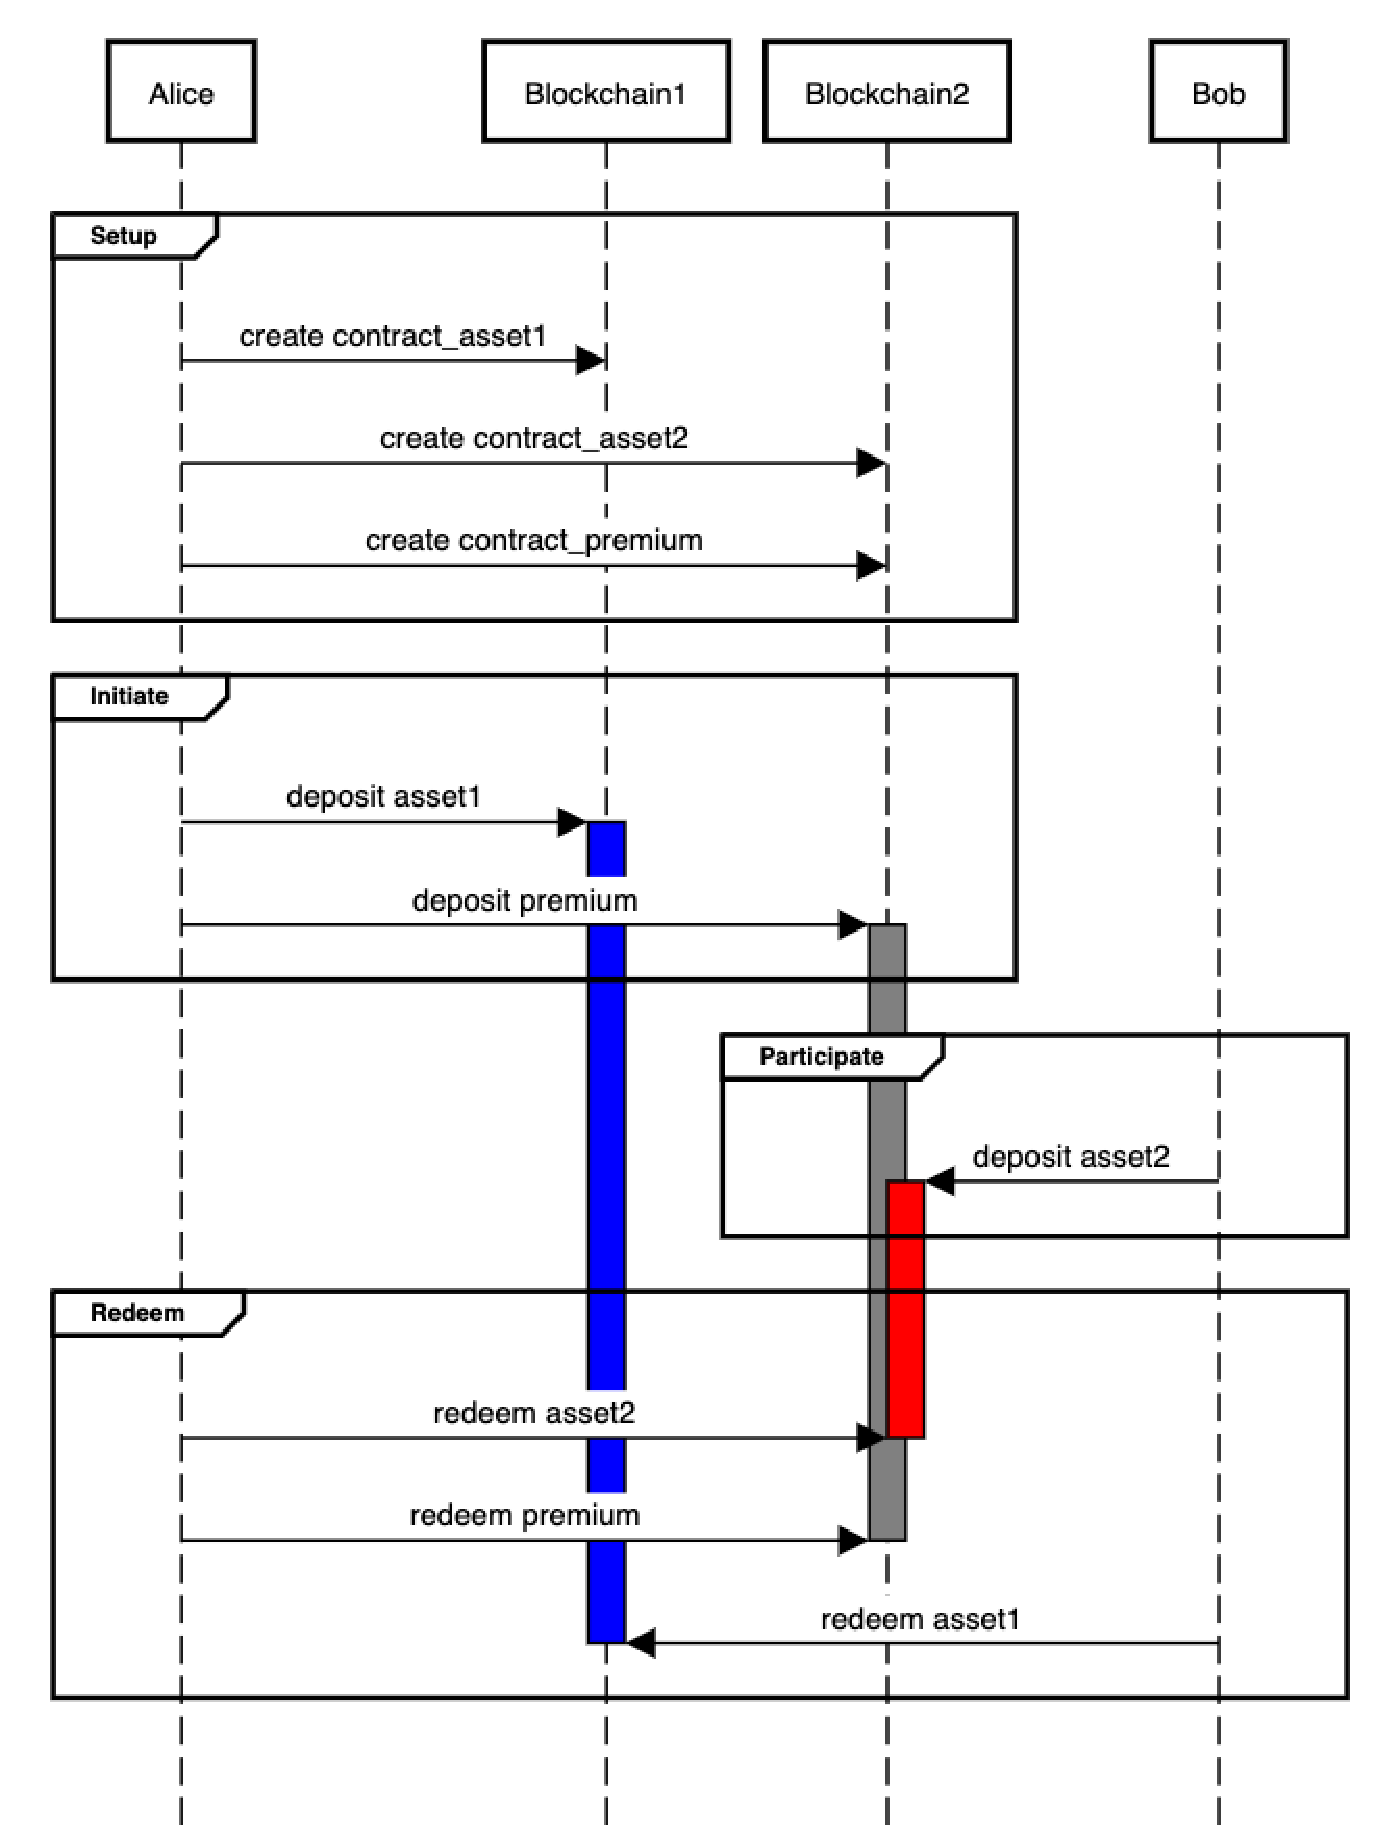
\includegraphics[width=\textwidth]{sequence_diagram_currency_exchange.eps}
        \caption{Sequence diagram of the currency exchange-style Atomic Swap.}
        \label{fig:sequence_diagram_currency_exchange}
    \end{subfigure}
    \quad
    \begin{subfigure}{.3\textwidth}
        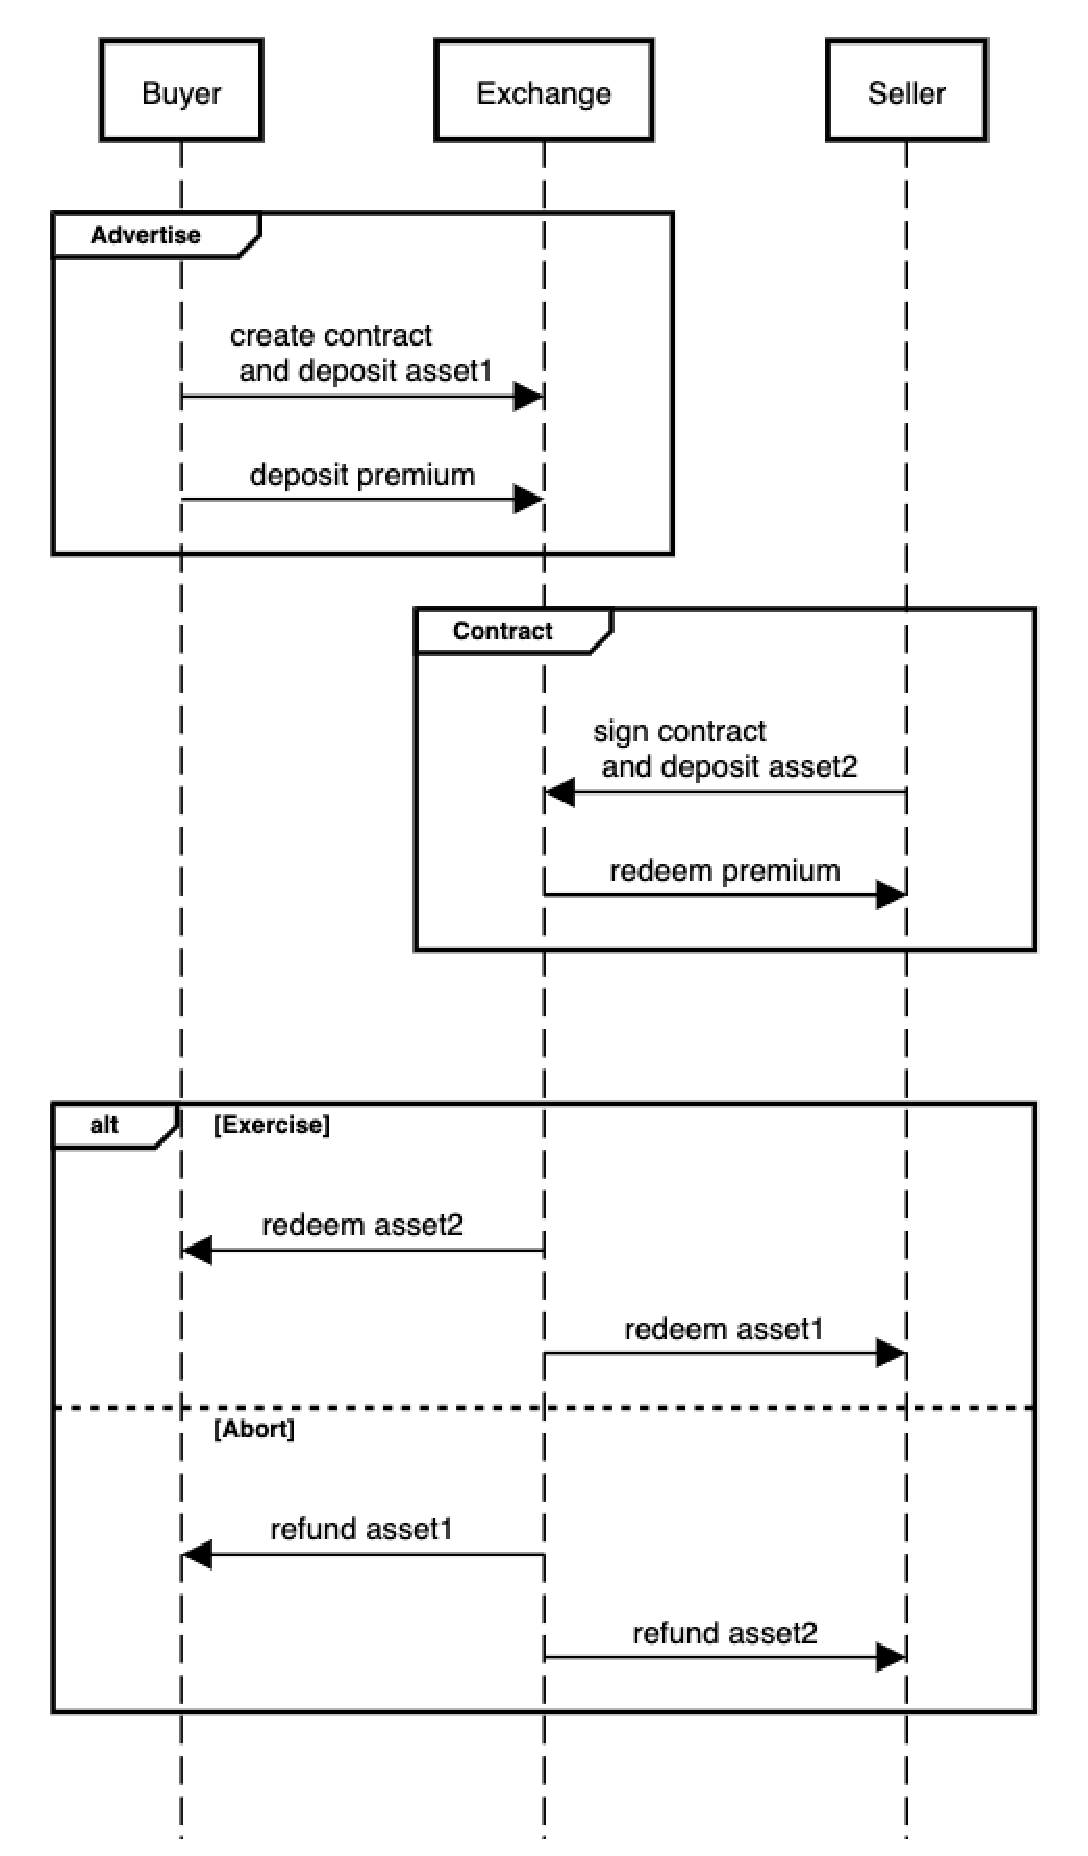
\includegraphics[width=\textwidth]{sequence_diagram_options.eps}
        \caption{Sequence diagram of the American Call Option-style Atomic Swap.}
        \label{fig:sequence_diagram_options}
    \end{subfigure}
\caption{Sequence diagrams.}
\label{fig:sequence_diagrams}
\end{figure*}

\end{document}
